%%%%%%%%%%%%%%%%%%%%%%%%%%%%%%%%%%%%%%%%%%%%%%%%%%%%%%%%
% Este é um documento que servirá de modelo para
% os relatórios feitos na disciplina Circuitos Digitais
% 2016-2
%%%%%%%%%%%%%%%%%%%%%%%%%%%%%%%%%%%%%%%%%%%%%%%%%%%%%%%%%

\PassOptionsToPackage{brazil,american}{babel}
\documentclass[12pt]{article}

\usepackage{sbc-template}
\usepackage[brazil,american]{babel}
\usepackage[utf8]{inputenc}

\usepackage{graphicx}
\usepackage{url}
\usepackage{float}
\usepackage{listings}
\usepackage{color}
\usepackage{todonotes}
\usepackage{algorithmic}
\usepackage{algorithm}
\usepackage{hyperref}
     
\sloppy

\title{Experimento 5\\ 
Circuitos Combinacionais: Conversão de Códigos}

\author{Isaac Lopes, 12/0120801\\
	Lucas Mafra Chagas, 12/0126443 \\
	Marcelo Giordano Martins Costa de Oliveira,  12/0037301
}


\address{Dep. Ciência da Computação -- Universidade de Brasília (UnB)\\
	CiC 116351 - Circuistos Digitais - Turma C
	\email{\{giordano.marcelo, chagas.lucas.mafra, isaaclopinho\}@gmail.com}
}

\begin{document} 

\maketitle

 \begin{abstract}
   In this report, it was designed an BCD code converter with 5bit using Quartus 13.01 software. 
 \end{abstract}
     
 \begin{resumo} 
  Nesse experimento, foi projetado um conversor de código de BCD com 5bits utilizando o software Quartus 13.01.
 \end{resumo}


\section{Objetivos}
\label{sec:Objetivos}

Estudo e projeto de conversores de código. O código de entrada utilizado como exemplo é o BCD e o de saída é um código de 5 bits. São apresentados, ainda, os códigos de Gray, excesso-3, biquinário e outros.

\section{Materiais} 
\label{sec:Materiais}

\begin{itemize}
    \item software Quartus II versão 13.0
    \item kit de desenvolvimento em FPGA DE2 Altera 
\end{itemize}


\section{Introdução}
\label{sec:Introducao}

A necessidade de realizar a comunicação entre dois sistemas digitais diferentes leva à criação de sistemas de interligação, que possui como função básica a conversão de códigos de um sistema para o outro.
Temos um código quando uma palavra X = {y1, y2, …,yn}, que é interpretada de certa maneira, é escrita de maneira diferente, X = {z1,z2,...,zn} e essa nova forma de escrita só é compreendida se a entidade que lê sabe como funciona o código. Um conversor de códigos é um tipo de circuito que pega a palavra X em sua forma original, escrita em um determinado código e a transforma. A palavra é a mesma mas a sua constituição é diferente, estando de acordo com um novo código.
É dito que um conversor é um codificador quando sua entrada representa um código que é ativado uma e somente uma linha de entrada por vez. Analogamente, é dito que um conversor é um decodificador quando sua saída representa um código que é ativado uma e somente uma linha de saída por vez. Por exemplo, um conversor é codificador e decodificador para códigos decimais.

O código BCD é um código muito comum. Este código é um código ponderado, ou seja, a cada bit é atribuído um peso. Portanto, números BDC podem ser convertidos para decimal da seguinte forma:

N = 8B{\tiny 3} + 4B{\tiny 2} + 2B{\tiny 1} + 1B{\tiny 0}

Onde Bi é igual ao valor 0 ou 1, i $\in {0,1,2,3}$. O código BCD é usado para representar apenas valores de 0 a 9.
O código 2 4 2 1 também é ponderado, como o BCD, mas os valores dos seus pesos são diferentes. O código Excesso de 3 não é ponderado pois temos que a representação dos valor é equivalente à sua representação somada de três em binário. O código biquinário é ponderado, com os pesos sendo 5043210.
O código de Gray é o código conhecido como código binário refletido. Ele é vantajoso pois dois valores consecutivos diferem em apenas 1 bit. Esse código é utilizado no mapa de Karnaugh.
O experimento relatado aqui trabalha com o código BCD e analisa o funcionamento de um conversor deste código.


\section{Procedimentos}
\label{sec:Procedimentos}

Nesse experimento tivemos que:

\begin{itemize}
	\item Obter as funções booleanas através do mapa de Karnaugh;
	\item Desenhar o diagrama lógico total usando o número mínimo de portas lógicas e realizar a simulação funcional e temporal;
	\item Desenhar o diagrama lógico total usando somente portas NAND de 2 e 4 entradas e realizar a simulação funcional e temporal;
	\item Sintetizar o conversor de códigos projetado com o número mínimo de portas lógicas.
		
\end{itemize}

\subsection{Funções booleanas através do mapa de Karnaugh}
\label{sec:karnaugh}

As funções booleanas obtidas para V, W, X, Y e Z foram obtidas através da análise dos minitermos de cada função, já que, para a implementação com portas NAND a utilização de minitermos é mais favorável. Temos portanto que:

$V= \overline{A}B\overline{C}D + \overline{A}BC\overline{D} + \overline{A}BCD + A\overline{BCD} + A\overline{BC}D$;

$W= \overline{A}B\overline{C D} + \overline{A}B\overline{C}D + \overline{A}BC\overline{D}  + \overline{A}BCD + \overline{A}BCD + A\overline{BCD}$;

$X = \overline{AB}CD + \overline{A}B\overline{C D} + \overline{A}B\overline{C}D + \overline{A}BC\overline{D} + \overline{A}BCD$;

$Y = \overline{A B}C\overline{D}+ \overline{A B}CD + \overline{A}B\overline{CD} + \overline{A}B\overline{C}D + \overline{A}BC\overline{D} $;

$Z = \overline{A B C}D + \overline{A B}C\overline{D}+ \overline{A B}CD + \overline{A}B\overline{C D} + \overline{A}B\overline{C}D + \overline{A}BC\overline{D} $;

Como estamos codificando valores em código BCD, temos que os valores de 10 a 15 são don’t cares. Portanto, em todos os mapas de Karnaugh apresentados abaixo, temos um ‘X’ marcado nas casas do mapa referentes a estes valores.

\begin{figure}[H]
	\centering
	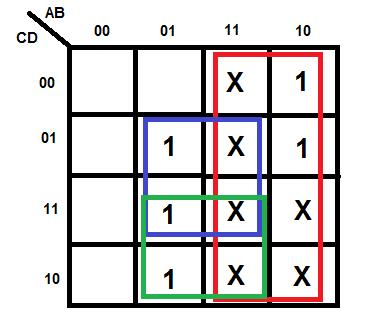
\includegraphics[width=.5\textwidth]{mapakarnaughv.png}
	\caption{Mapa de Karnaugh da função V}
	\label{fig:karnaughv}
\end{figure}

$ V = A + BC + BD$

\begin{figure}[H]
	\centering
	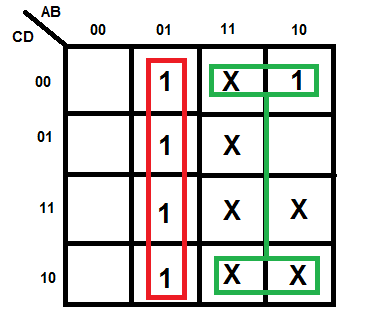
\includegraphics[width=.5\textwidth]{mapakarnaughw.png}
	\caption{Mapa de Karnaugh da função W}
	\label{fig:karnaughw}
\end{figure}

$ W = B + A\overline{D}$

\begin{figure}[H]
	\centering
	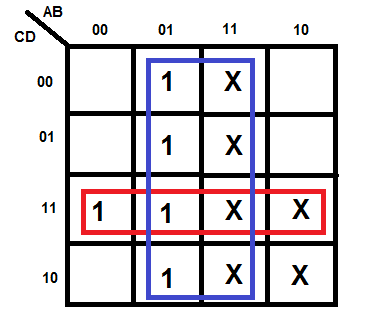
\includegraphics[width=.5\textwidth]{mapakarnaughx.png}
	\caption{Mapa de Karnaugh da função X}
	\label{fig:karnaughx}
\end{figure}

$ X = B + CD$

\begin{figure}[H]
	\centering
	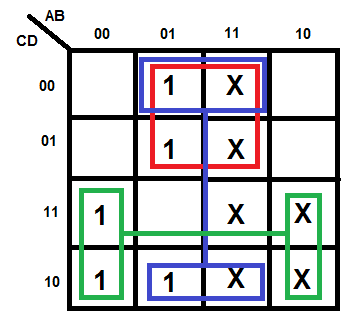
\includegraphics[width=.5\textwidth]{mapakarnaughy.png}
	\caption{Mapa de Karnaugh da função Y}
	\label{fig:karnaughy}
\end{figure}

$ Y = \overline{B}C + B\overline{C} + C\overline{D}$

\begin{figure}[H]
	\centering
	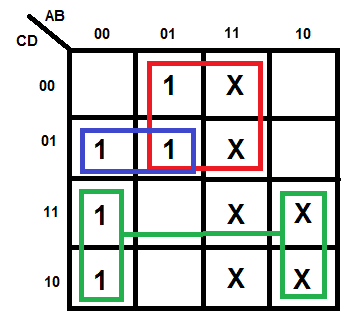
\includegraphics[width=.5\textwidth]{mapakarnaughz.png}
	\caption{Mapa de Karnaugh da função Z}
	\label{fig:karnaughz}
\end{figure}

$ Z = \overline{B}C + B\overline{C} + \overline{A}\overline{B}D$

\subsection{Diagrama lógico total usando o número mínimo de portas lógicas}
\label{sec:minimoporta}

\subsection{Diagrama lógico total usando somente portas NAND de 2 e 4 entradas}
\label{sec:nandporta}

\subsection{Conversor de códigos projetado com o número mínimo de portas lógicas}
\label{sec:conversor}

Desenvolvemos no kit de desenvolvimento em FPGA DE2 Altera o código projetado com o número mínimo de portas lógicas. É possível ver o resultado no seguinte link: \href{https://www.youtube.com/watch?v=1CFXa6bdLcs}{Vídeo no Youtube}



\section{Análise dos Resultados}
\label{sec:Resultados}


\section{Conclusão}
\label{sec:Conclusao}

O experimento tornou possível perceber a utilidade de conversores na interface entre sistemas digitais. A implementação desses conversores utilizando circuitos combinacionais foi muito interessante de ser feita, além de ter sido concluída com sucesso. Também foi possível ver, mais uma vez, que as portas NAND são de extrema importância na construção de circuitos digitais, inclusive os conversores,já pela rapidez oferecida por essa porta.


\bibliographystyle{sbc}
\bibliography{relatorio}


\newpage 
% Colocar aqui apenas as respostas dos itens da Auto-Avaliação
\section*{Auto-Avaliação}

\begin{enumerate}
    \item b
    \item a
    \item c
    \item d
    \item a
    \item a
\end{enumerate}


\end{document}
